\chapter{Sample-level CNN using raw waveforms}
by Thorsten Wünsche

\bigskip

In this chapter, we attempt to recreate an approach that reduces preprocessing by working with raw waveforms directly. Section \ref{sec:theory} presents the original paper and discusses the theory behind it. In section \ref{sec:development} we discuss the development process up until the first working prototype. Experiments and improvements to our own version are described in section \ref{sec:experiments}. Finally, section \ref{sec:conclusion} summarizes our experiences with this approach.

\section{Theory and original paper}
\label{sec:theory}

"Sample-level Deep Convolutional Neural Networks for Music Auto-tagging Using Raw Waveforms" \cite{DBLP:journals/corr/LeePKN17} by Jongpil Lee, Jiyoung Park, Keunhyoung Luke Kim, Juhan Nam

\begin{center}
	\begin{tabular}{ c c c c}
		
		layer & stride & output & \# of params\\
		\hline
		\hline
		conv 3-128 & 3 & 19683 x 128 & 512 \\
		\hline
		conv 3-128 & 1 & 19683 x 128 & 49280 \\
		maxpool 3 & 3 & 6561 x 128 & \\
		\hline
		conv 3-128 & 1 & 6561 x 128 & 49280 \\
		maxpool 3 & 3 & 2187 x 128 & \\
		\hline
		conv 3-256 & 1 & 2187 x 128 & 98560 \\
		maxpool 3 & 3 & 729 x 256 & \\
		\hline
		conv 3-256 & 1 & 729 x 256 & 196864 \\
		maxpool 3 & 3 & 243 x 256 & \\
		\hline
		conv 3-256 & 1 & 243 x 256 & 196864 \\
		maxpool 3 & 3 & 81 x 256 & \\
		\hline
		conv 3-256 & 1 & 81 x 256 & 196864 \\
		maxpool 3 & 3 & 27 x 256 & \\
		\hline
		conv 3-256 & 1 & 27 x 256 & 196864 \\
		maxpool 3 & 3 & 9 x 256 & \\
		\hline
		conv 3-256 & 1 & 9 x 256 & 196864 \\
		maxpool 3 & 3 & 3 x 256 & \\
		\hline
		conv 3-512 & 1 & 3 x 512 & 393728 \\
		maxpool 3 & 3 & 1 x 512 & \\
		\hline
		conv 1-512 & 1 & 1 x 512 & 262656 \\
		dropout 0.5 & - & 1 x 512 & \\
		\hline
		sigmoid & - & 50 & 25650 \\
		
		& & & \\	
	\end{tabular}
	\label{tab:sample-dcnn_original-model}
	\captionof{table}{The original model with the parameters Jongpil Lee, Jiyoung Park, Keunhyoung Luke Kim and Juhan Nam found the most successful. The layer "conv3-128 maxpool3" is to be understood as a one dimansional convolutional layer with filter length 3 producing 128 filters, followed by a maxpool layer with pooling length 3. The 50 in the sigmoid layer is the number of labels in the corresponding dataset.}
\end{center}


\section{Development and limitations}
\label{sec:development}

\begin{figure}[!htb]
	\centering
	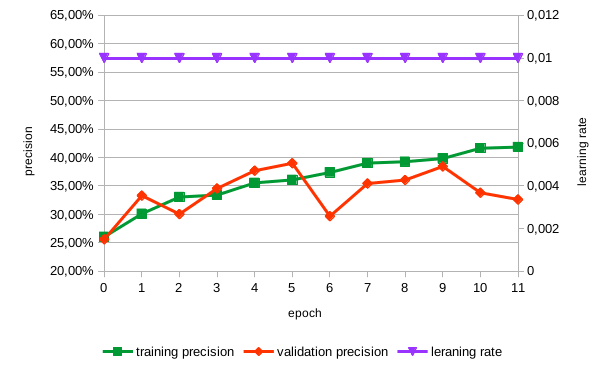
\includegraphics[width=.9\linewidth]{images/sample-dcnn-m3-n9-seg10-128_512-plateau.png}
	\caption{Performance of the $3^9$ model using 10 segments of music, between 128 and 512 filters and a reduce on plateau learning rate with the parameters suggested in the paper.}
	\label{fig:sample-dcnn-m3-n9-seg10-128_512-plateau}
\end{figure}


We created our own prototype by recreating the most successful model found by Jongpil Lee, Jiyoung Park, Keunhyoung Luke Kim and Juhan Nam. Their $3^9$ model shown in table \ref{tab:sample-dcnn_original-model} uses a one dimensional filter of size three in a convolutional neural network of depth 9 (1+9+1).  Using a frame-size of three, this model converts 59049 samples into 19683 frames. We also use the same sample size (22050 Hz), so that each input into the model covers 2678 ms of audio.

The large FMA dataset would not only take far too long to train on a desktop computer, but is also too large to be stored on the available hard drives. Therefore ee use the small version of the dataset with 8000 songs (30 s each) to adjust our model, before we attempt to classify the larger version on a server. Some of the files in the small dataset are corrupt or too short, where not enough data for our model is available, the tensors are filled ip with random numbers. As the defect files are in the single digits, this should not have a noticeable effect on the performance.

The performance of our initial implementation is shown in figure \ref{fig:sample-dcnn-m3-n9-seg10-128_512-plateau}. The learning rate scheduler does not seem to work as intended and possibly due to a constant learning rate of $0.01$, the accuracy leaves a lot to be desired. Even with these limitations, the model reaches an accuracy of 25\% on both the training and the validation set after a single epoch. In a balanced dataset with eight classes, this is already twice as good as a naive approach. The precision on both sets rises by 10-15 percentage points, though the validation precision declines soon after. All in all, this prototype works, but will need to be adapted to our hardware and time limitations.


\section{Experiments}
\label{sec:experiments}

Next, we will tweak the prototype described in section \ref{sec:development}. This will involve changing hyperparameters as well as the filter-length and depth of the model. Using a desktop computer with eight virtual cores and a GeForce GTX 1060 6GB, the training of the prototype completed 12 epochs within eight hours. The following experiments are all limited to this same timespan. This does mean that the model may not fully converge, but our primary concern is finding modifications that can increase the performance of our model before training it on the larger dataset using more capable hardware. 

\subsection{Learning rate}

\label{subsec:learning_rate}
\begin{figure}[!htb]
	\centering
	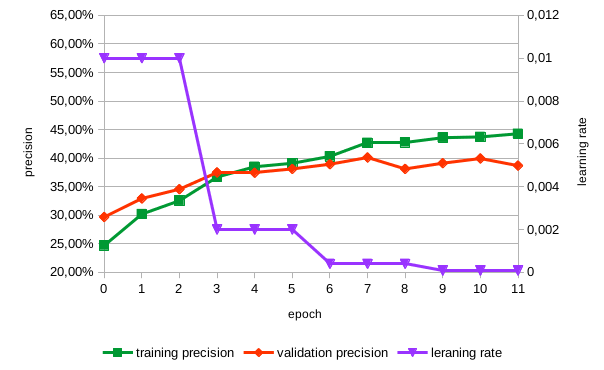
\includegraphics[width=.9\linewidth]{images/sample-dcnn-m3-n9-seg10-128_512-step.png}
	\caption{Performance of the $3^9$ model using 10 segments of music and between 128 and 512 filters. This version was modified to use a step learning rate dividing by a factor five every three epochs.}
	\label{fig:sample-dcnn-m3-n9-seg10-128_512-step}
\end{figure}

The first subject of experimentation is the learning rate. In the original prototype, we use the same model as Jongpil Lee, Jiyoung Park, Keunhyoung Luke Kim and Juhan Nam: The learning rate starts at $0.01$ and decreases by a factor five when the validation loss has not increased in three consecutive epochs. In eight hours of training on a desktop computer, our prototype finished 12 epochs. This means that a quarter of the total training time would be required to identify a plateau. Indeed, during our initial training the learning rate was not reduced even once. With more time or faster hardware, this would be acceptable. We want to conduct a few other experiments as well however, and therefore tried two other approaches.

First, we keep the starting rate of $0.01$ and reduce it by the same factor five after three epochs regardless of the validation error. This leads to three decreases over the course of one session. In the paper, training was halted after four decreases.

As can be seen in figure \ref{fig:sample-dcnn-m3-n9-seg10-128_512-step}, the precision on the validation set with our modification not only rises above 40\% at one point, it also remains much more stable, making it an overall improvement. The downside of this approach is, that after a few more epochs, the learning rate will be too low to allow for further improvement, even if the model and the dataset still had potential. As we plan to also apply our model to a larger dataset on more powerful hardware, this schedule might prove too limiting.

To adjust the learning rate in a more flexible manner, we return to the reduce on plateau scheduler, but make some adjustments to allow it to be effective even with limited time and hardware. We reduce the patience period from three to zero, reducing immediately upon a rise in the validation error.As this makes the scheduler more vulnerable to small mistakes, we reduce the factor of the division from five to two and add a one epoch cooldown, to give the validation error time to recover after the learning rate has been reduced. The results are shown in figure \ref{fig:sample-dcnn-m3-n9-seg10-128_512-plateau_mod}. The validation precision is initially less stable, but ends up at similar values to the previous experiment, while the precision on the training set rises to above 50\%. Most importantly, this scheduler adapts itself to the dataset and slows down only when required, rather than at a constant and possibly too high speed.

We conclude, that our modified version of the reduce on plateau scheduler is an improvement on our limited hardware and will use this version in all experiments from here on out. On more powerful hardware however, the original version will likely be superior, as it is less susceptible to small fluctuations in the validation error.




\begin{figure}[!htb]
	\centering
	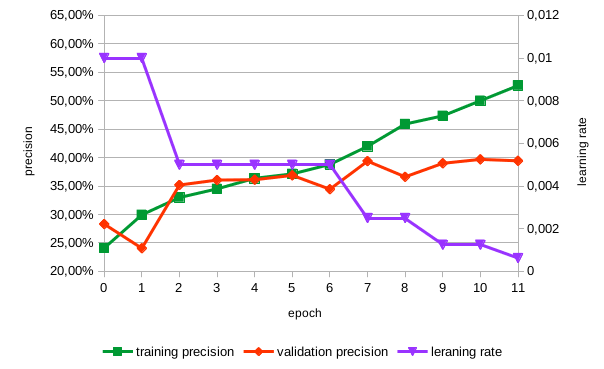
\includegraphics[width=.9\linewidth]{images/sample-dcnn-m3-n9-seg10-128_512-plateau_mod.png}
	\caption{Performance of the $3^9$ model using 10 segments of music and between 128 and 512 filters. This version was modified to use a reduce on plateau learning rate dividing by a factor 2 after every epoch, in which the validation loss did not fall. After every reduction, there is a one epoch cooldown to give the loss a chance to recover.}
	\label{fig:sample-dcnn-m3-n9-seg10-128_512-plateau_mod}
\end{figure}
\subsection{Number of filters}

In the paper, the authors experiment both on MTAD and MSD. For MTAT, increasing the number of filters in the convolution layers from 16 to 512 is sufficient, but performance on MDS improves when starting at 128 filters. Our prototype uses 128-512 filters initially, in this experiment, we reduce the number of filters in the earlier layers to 16 and gradually raise the number to 512. If this method results in a reduced training time without sacrificing accuracy, then the increased number of epochs may make up for the somewhat lower complexity.

\begin{figure}[!htb]
	\centering
	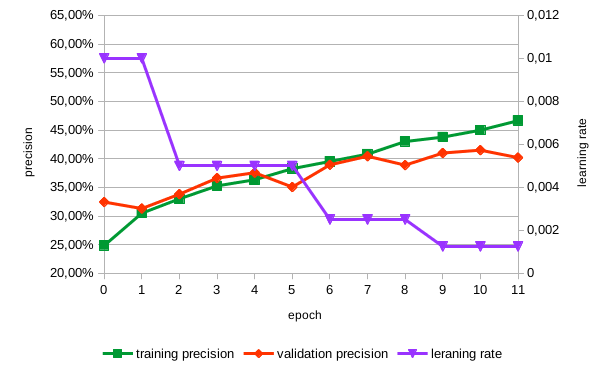
\includegraphics[width=.9\linewidth]{images/sample-dcnn-m3-n9-seg10-16_512-plateau_mod.png}
	\caption{Performance of the $3^9$ model using 10 segments of music and the modified reduce on plateau learning rate described in subsection \ref{subsec:learning_rate}. This version uses a reduced number of filters, increasing from 16 to 512 rather than 128 to 512.}
	\label{fig:sample-dcnn-m3-n9-seg10-16_512-plateau_mod}
\end{figure}

After training the model for eight hours, no significant decrease in training time was found. As shown in figure \ref{fig:sample-dcnn-m3-n9-seg10-16_512-plateau_mod}, the accuracy on the validation set however grew slightly, while the training precision fell significantly. This would suggest, that our previous model was overfitting to a small degree. Therefore we will keep using the reduced number of filters on the small dataset (8000 samples), but will increase it back to full for more complex applications.



\subsection{Number of segments}
\begin{figure}[!htb]
	\centering
	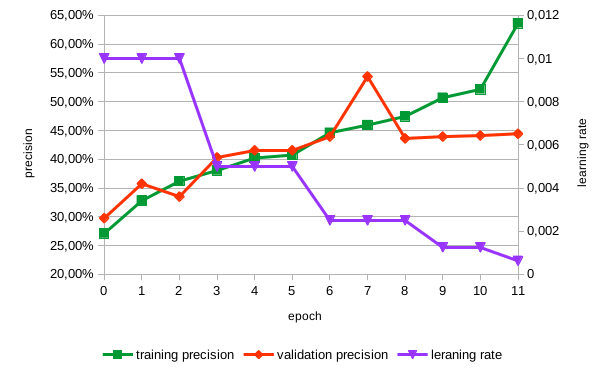
\includegraphics[width=.9\linewidth]{images/sample-dcnn-m3-n9-seg1-16_512-plateau_mod.png}
	\caption{Performance of the $3^9$ model using the modified reduce on plateau learning rate and a reduced number of filters, increasing from 16 to 512 rather than 128 to 512. This Version trains ans classifies only one segment of music at a time.}
	\label{fig:sample-dcnn-m3-n9-seg1-16_512-plateau_mod}
\end{figure}

\subsection{Depth and filter length}

\section{Conclusion}
\label{sec:conclusion}